% ======================================================================
\section{Introduction}

This document provides a guide to the \VRO\ approach to work management and annual planning.
See the operations proposal \gls{RDO}-018 for a description of the full scope and high level goals of the program.
There is no formal \gls{EVMS} required from the funding Agencies (the \gls{National Science Foundation} (\gls{NSF}) and the \gls{Department of Energy} (DOE) Office of Science) so activities are planned in detail on a semi-annual basis and effort towards that schedule of activities is tracked through an agile process.

The annual planning process starts by reviewing, revising, and adding major milestones to the next fiscal year plan.
These are centered around releasing data to the public and major maintenance to the telescope system once we enter the phase of full survey operations, and it's these major milestones that are tracked and reported on in the annual \gls{NOIRLab} Program Operations Plan (\gls{POP}) and \gls{SLAC} Field Work Proposal (FWP).
Then, on a six-month \gls{cycle}, the Leadership Team builds a series of ``epic'' milestone activities that are discrete pieces of work within Departments and Teams to collectively deliver the high level milestones.
Teams record their day to day work in \gls{JIRA} and overall progress is monitored automatically through Smartsheet and reported to the Agencies through our managing organizations.

This framework allows the multidisciplinary Rubin teams to operate the facility and generate nightly data products while continuously improving efficiency of workflows,
as well as iteratively responding to user community feedback on a longer timescale to maximize the scientific benefit of annual data releases.
Examples include optimizing the observing strategy as the survey progresses, improving algorithms in response to the user community feedback,
and other incremental work needed to produce the annual data releases.

In this document, we lay out the procedural details for how we define and carry out annual plans, effectively track work progress to ensure delivery of milestones, maintain visibility in our workflows, remain responsive to change, and offer staff the ability to innovate and collaborate.


% ======================================================================
\section{Organizational Structure}
\label{sec:structure}

\subsection{Rubin \gls{Operations} Leadership}
\label{sec:contacts}

Rubin Observatory is a Program of \gls{NSF}'s \gls{NOIRLab}.
The Rubin Observatory \gls{Director} is Robert Blum, the Rubin Deputy \gls{Director} for \gls{NOIRLab} is currently under recruitment, and the Rubin Deputy \gls{Director} for \gls{SLAC} is Phil Marshall.
They are the first point of contact for all issues regarding project management within \RO \gls{Operations}.

The Head of \gls{Operations} is Ranpal Gill and the Program Coordinator is Cathy Petry.
They monitor the budget and maintain details within the \gls{NOIRLab} accounting system.
They assist in developing the annual Program Operating Plan (\gls{POP}), tracking milestones and reporting on progress.

On the \gls{SLAC} side, Christine Soldahl is the \gls{Business Manager} who handles similar tasks.

Rubin Operations has four operational Departments in addition to the RDO (Rubin Director’s Office): \gls{ROO} (Rubin Observatory Operations), \gls{RDP} (Rubin Data Production), \gls{RPF} (Rubin System Performance), and REO (Rubin Education and Public Outreach).
Each operational Department is led by an Associate \gls{Director} (\gls{AD}).

\subsection{Annual Reporting}
\label{sec:reporting}

The \gls{POP} is a defined process for \gls{NOIRLab}, where annually the next fiscal year's \gls{POP} is developed and reporting on progress of the current year's \gls{POP} to the \gls{NSF} is done quarterly with a final annual progress report.
Rubin Operations considers the \gls{POP} to be a Rubin activity, which informs both \gls{NOIRLab} and \gls{SLAC} leadership of the annual Rubin activity including milestones and budget.
For \gls{NOIRLab}, the Rubin \gls{POP} is integrated and delivered to \gls{NSF} for the next fiscal year at the end of the current fiscal year.
For \gls{SLAC}, the \gls{POP} informs \gls{SLAC}'s annual planning, which culminates in a Field Work Proposal (\gls{FWP}) for all \gls{SLAC} High Energy Physics activity including Rubin.

The \gls{FWP} is delivered in June of the current fiscal year, and covers the federal budget request for the next two fiscal years.
The \gls{FWP} is previewed to \gls{SLAC} management and \gls{DOE} in February in advance of the final delivery in June.
Because the \gls{POP} for NSF lags the FWP for DOE by one year, and their submission dates differ by several months, Rubin does high level planning in early \gls{Q2} of the fiscal year (January and February) and plans 2 years ahead, as required for the \gls{SLAC} FWP.
Detailed activity planning, including defining smaller chunks of work as lower level milestones, continues though the year in advance of the next year.
This detailed activity planning is the subject of this document.

\subsection{Work Breakdown Structure}
\label{sec:wbs}

The \gls{WBS} is a hierarchical description of \gls{Rubin Operations} from an activity-based perspective.
It provides a useful structure to organize \gls{Rubin Operations} and plan annual work around.
Rubin is level 1 of the \gls{WBS}, the departments are level 2, and teams within the departments are level 3 and in the case of Program \gls{Operations}, level 4.
Individual roles in operations are defined at the lowest level.
% In the Planning Google sheets there is no level 4 as there is in the budget table in the Proposal, but there is a direct mapping in that it's rolled up.  We can decide whether to change the google tools to match the proposal budget tables (will help later with reconcilation), or we can make the mapping clearly described.  Also, in Google sheets 1.10 and 1.11 are rolled into Program Operations, and they are separate elements in this table, and in the budget tables.

This table shows the level 2 and level 3 elements of the \gls{Rubin Operations} work breakdown structure.

% We want to add the next level down in this tables (include Teams). No need to refer to NOIRLab's WBS for Rubin.
% Teams have been added as extra rows with an extra column for delineation, but there might be a better presentation format.

% This table is not auto-numbered and the next table is numbered "3" so this will have to be figured out.

% \begin{table}
\begin{longtable}[]{@{}lll@{}}

\hline
L2 \gls{WBS} & \gls{L3} \gls{WBS} & Description \tabularnewline
\hline
\endhead

1 & & Rubin \gls{Director}'s Office  \tabularnewline
  & 1.1 & \hspace{0.5cm} \gls{Director}'s Office  \tabularnewline
  & 1.2 & \hspace{0.5cm} \gls{Safety}  \tabularnewline
  & 1.3 & \hspace{0.5cm} Program \gls{Operations}\footnotemark[1]  \tabularnewline
%  & 1.3.1 & Program Operations  \tabularnewline
%  & 1.3.2 & Administrative Operations  \tabularnewline
%  & 1.3.3 & Portfolio Management  \tabularnewline
%  & 1.3.4 & Communications  \tabularnewline
%  & 1.3.5 & Document Management  \tabularnewline
%  & 1.3.6 & 5-Year Planning  \tabularnewline
  & 1.4 & \hspace{0.5cm} In-Kind Program Coordination  \tabularnewline
  & 1.8 & \hspace{0.5cm} Legacy Survey of Space and Time  \tabularnewline
  & 1.10 & \hspace{0.5cm} Sustainability  \tabularnewline
  & 1.11 & \hspace{0.5cm} Site Protection  \tabularnewline
  & 1.12 & \hspace{0.5cm} Rubin Site Protection  \tabularnewline
2 & & Rubin Observatory \gls{Operations}  \tabularnewline
  & 2.1 & \hspace{0.5cm} Observatory \gls{Operations} Management  \tabularnewline
  & 2.2 & \hspace{0.5cm} Observatory Science \gls{Operations}  \tabularnewline
  & 2.3 & \hspace{0.5cm} Observatory Software  \tabularnewline
  & 2.4 & \hspace{0.5cm} \gls{Summit} \gls{Operations}  \tabularnewline
  & 2.5 & \hspace{0.5cm} Nighttime \gls{Operations}  \tabularnewline
  & 2.6 & \hspace{0.5cm} Engineering  \tabularnewline
3 & & Rubin Data Production \tabularnewline
  & 3.1 & \hspace{0.5cm} Data Production Management  \tabularnewline
  & 3.2 & \hspace{0.5cm} Infrastructure and Support  \tabularnewline
  & 3.3 & \hspace{0.5cm} Data and Processing Architecture  \tabularnewline
%   & 3.4 & Execution (disabled)  \tabularnewline
  & 3.5 & \hspace{0.5cm} Algorithms and Pipelines  \tabularnewline
  & 3.6 & \hspace{0.5cm} Service Quality and Reliability Engineering  \tabularnewline
  & 3.7 & \hspace{0.5cm} DevOps Support  \tabularnewline
  & 3.8 & \hspace{0.5cm} Data Security  \tabularnewline
4 & & Rubin System Performance  \tabularnewline
  & 4.1 & \hspace{0.5cm} System Performance Management  \tabularnewline
  & 4.2 & \hspace{0.5cm} \gls{Verification} and \gls{Validation}  \tabularnewline
  & 4.3 & \hspace{0.5cm} Community Engagement  \tabularnewline
  & 4.4 & \hspace{0.5cm} Survey Scheduling  \tabularnewline
  & 4.5 & \hspace{0.5cm} \gls{Systems Engineering}  \tabularnewline
5 & & Rubin \gls{Education and Public Outreach} \tabularnewline
  & 5.1 & \hspace{0.5cm} \gls{EPO} Management  \tabularnewline
  & 5.2 & \hspace{0.5cm} \gls{EPO} Technical  \tabularnewline
  & 5.3 & \hspace{0.5cm} Education  \tabularnewline
  & 5.4 & \hspace{0.5cm} Outreach  \tabularnewline

\hline

% footnote text
\footnotetext[1]{Program \gls{Operations} is made up of several groups at level 4 that are not presented here but are available for activity planning and budgeting.}
\end{longtable}
% Using a caption needs the "table" environment currently commented
% \caption{The level 2 and level 3 elements of the Rubin Operations work breakdown structure.}
% \label{tab:wbs}
% \end{table}

%\subsection{The Control Account Manager}
%\label{sec:cam}

Detailed work is planned in advance of each fiscal year at the team level.
Team leads will work with department associate directors to develop plans for activities that address specific milestones, projects, and level of effort activity.
Progress towards the highest level milestones is reported regularly throughout the fiscal year to \gls{SLAC}, \gls{AURA}, NSF and \gls{DOE}.


\subsection{Activity Types}
\label{sec:loe}

There are two types of activities (or epics) that are planned:  activities that result in a deliverable, and level of effort (or support) activities.
Progress can be tracked on activities with a deliverable by computing the fraction of the effort that is complete (percent complete) based on completed stories linked to the \gls{epic}.
Progress on \gls{LOE} work is assumed to progress proportionally with the passage of time.

\gls{LOE} activities include attending meetings, reporting on milestones, or taking part in other activities which do not directly map to a deliverable or product.
This may be particularly the case for technical managers or others in leadership roles.
In general, we strive to minimize the fraction of effort which is devoted to \gls{LOE} activities and favor those which are more directly accountable.
However, in certain cases such as operations and maintenance of telescope and facility systems, pipelines or other systems, \gls{LOE} is perfectly acceptable.
Technical staff in Chile at the summit facility may spend a much more significant fraction of time as \gls{LOE}.
As an example, a first-order estimate is that developers will spent 30\% of their time on \gls{LOE} type activities, and the remaining 70\% of their effort is planned and tracked against well-defined deliverables.


% ======================================================================
\section{Estimating Effort}
\label{sec:effort}

\subsection{Basic Assumptions}

% Note: These calculations are true for Construction but need to be updated for Rubin Operations since NOIRLab uses 1744 hours per year (83%) for scientists, scientists could have 20% or 50% for research, and research time and Training, Admin & DEI time is charged to RSS.  For Engineers, Training, Admin & DEI time is charged to ES.
% We could also refer to the effort planning tool Phil has made ("Team Effort Planner" in Staffing Plan).  Right now, most people have "Commenter" permission in the STaffing Plan workbook and this is not sufficient to use the dropdown filter that TLs and ADs would need to use this tool.  We could move this to a stand-alone workbook.

Rubin \gls{Operations} assumes that a full-time individual works for a total of 1,800 hours per year: this figure is \emph{after} all vacations, sick leave, etc are taken into account.
The \gls{Rubin Operations} partners, \gls{SLAC} and \gls{NOIRLab}, may have different definitions for tracking their staff time; \gls{Rubin Operations} uses 1,800 hours per year as a fiducial value for effort estimation purposes.

In general, staff in \gls{Rubin Operations} roles at a given expected full-time equivalent (\gls{FTE}) effort level are expected to devote that fraction of their total work time to \RO.

Staff in ``scientist'' or ``engineer'' roles can allocate up to 2\% of their time to training, 2\% to administrative activities and 1\% to outreach and \gls{DEI} activities.
% I have heard it said that staff has up to 3% for Outreach and DEI but I don't know how that resolves to the budget numbers described in the previous sentence
% Perhaps we just roll it all up into 5%, but it's a good place to reiterate that staff *are expected* to spend time on DEI

Staff in ``scientist'' roles are expected to spend 20\% of their time on personal research (see the \gls{Rubin Operations} Plan for details).
That is, scientists are expected to devote 1,440 hours per
year to operations activity, and the remainder of their time to personal research.
% Some scientists are 50%

% Confirmation on how we will be having staff charge for ES/RSS budgeted time in FY22 will be needed.  One suggestion is to not worry about this until FY23 when staff are contributing more than 50% of their time to NOIRLab.
Personal research time is charged to a \gls{NOIRLab}'s Research and Science Services (\gls{RSS}) project code and is prorated for staff who are fractionally allocated to \gls{Rubin Operations}.
Training, administrative, and outreach and \gls{DEI} time is charged to either RSS or \gls{ES} depending on where staff will move into \gls{NOIRLab} (RSS or \gls{ES}).
Functional Managers will ensure the proper project codes are available on your timecard.

Rubin expects to pay the full rate for any scientist or engineer who contributes full-time or fractionally to operations.
This is handled through indirect rates at \gls{NOIRLab} and direct charges to research accounts at \gls{SLAC}.
Science time is included in the subcontracts of our partners at affiliated institutions through indirect charges
similar to the case for \gls{NOIRLab}.

In Data Production, the base assumption is that 30\% of an individual's \RO operations time (i.e. 540 hours/year for a full-time developer, 432 hours/year for a full-time scientist) are devoted to
overhead for regular meetings\footnote{``Meetings'' include, for example, scheduled weekly team meetings, stand-ups, etc;
major conferences or project meetings involving preparation, travel time, etc should be scheduled in advance and allocated \glspl{SP}.},
ad-hoc discussions and other interruptions.
This work is counted as \gls{LOE}.
It is actively encouraged to allocate less than 30\% of an individuals time to \gls{LOE} where that is possible.

Assuming no variation throughout the year, we therefore expect 105 hours of productive work from a developer, or 84 hours from a scientist, per month.
Note that this is averaged across the year: some months, such as those containing major holidays, will naturally involve less working time than others: the remainder will necessarily include more working time to compensate. For other staff, the \gls{LOE} will be higher but include much more day to day activity than for the developer case.

Rather than working in hours, our \gls{JIRA} based system uses Story Points (\gls{SP}), with one \gls{SP} being defined as equivalent to four hours of effort (half a day's work) by a competent developer.

Thus, we expect developers and scientists to produce 26.25 and 21 \glspl{SP} per \emph{average} month respectively.

\begin{table}
\begin{longtable}[]{@{}lrrr@{}}
\hline
          & \multicolumn{2}{c}{Hours} & \multicolumn{1}{c}{\glspl{SP}} \\
          & Per year & Per month      & Per month \\
\hline
Full-time Developer & 1800     & 105            & 26.25 \\
Full-time Scientist & 1440     &  84            & 21.00 \\
\hline
\end{longtable}
\caption{Expected working rates for developers and scientists. Technicians and engineers follow the same rates as developers.}
\label{tab:working-rate}
\end{table}

\subsection{Special Cases}

\subsubsection{Newcomers}
\label{sec:newcomers}

New or inexperienced developers, even when devoting their full attention to \gls{story}-pointed work, will likely be less productive than their more experienced peers.
In this case, the ratio of hours to \glspl{SP} increases, but the number of hours remains constant.

Note that specific activities related to ``onboarding'' and getting up to speed with operations can be ticketed as regular work.
For example, working through tutorials, reading documentation, and so on are all activities which can earn \glspl{SP}.

\subsubsection{Team Leads and other Leadership Roles}

Individuals in leadership roles may find it necessary to assign a larger fraction of their time to \gls{LOE} type work, and therefore spend fewer hours generating \glspl{SP}.
The ratio of hours to \glspl{SP} remains constant, but the number of hours decreases.

% ======================================================================
\section{Long Term Planning}
\label{sec:long-term-plan}

\subsection{Timeline for Annual Planning}
\label{sec:annual-planning-timeline}

Our basic annual timeline is laid out below; for more detail on the budget planning and sandboxing, see Section~\ref{sec:annual-cycle}.

\begin{itemize}
\item December-March: accumulate top-down input for next year budget and schedule.
   \begin{itemize}
      \item Update lab-wide budget models (\gls{RAS}) from Staffing and Nonlabor plans, for quarterly forecasting (December, March).
      \item Update budget tools with any major changes, for \gls{AURA} \gls{NICRA} proposal. Incorporate any changes in \gls{SLAC} overhead rates and escalations.
      \item Adjust major milestone dates as events unfold.
   \end{itemize}
\item March
   \begin{itemize}
      \item Semi-annual process of planning epics and L3s for next six months
   \end{itemize}
\item April-May: \gls{NOIRLab} \gls{POP} process and \gls{SLAC} FWP development kick off mid-April, with major milestones and budget due end of May.
   \begin{itemize}
      \item Early April: set next \gls{FY} major milestones
         \begin{itemize}
            \item ADs review and/or add/edit major milestones
            \item Discuss in Ops Exec
            \item Implement changes in Smartsheet and \gls{JIRA}
         \end{itemize}
      \item Late April: set next \gls{FY} (and \gls{FY}+2) budget:
         \begin{itemize}
            \item Early April: freeze planning tools (\gls{WBS} and Cost Calculator)
            \item Joint agency operations status review (\gls{JOR})
            \item \gls{RDO} issues departmental budget guidance based on costed and reviewed plan.
         \end{itemize}
      \item May: next \gls{FY} Sandboxing:
         \begin{itemize}
            \item Early May: Prepare and issue sandbox workbooks, one per department.
            \item Early May Department management teams facilitate team-level sandbox pitches (including \gls{L2}/L3 milestons, changes to spending plans)
            \item Late May: Sandboxing Workshop, for all ops teams and \gls{Director}'s Office.
         \end{itemize}
   \end{itemize}
\item June-July: implement sandboxed changes.
   \begin{itemize}
      \item Implement proposed changes to Staffing Plan, \gls{Risk} Register, \gls{JIRA}/Smartsheet \gls{L2}/L3 milestones
      \item End of June: Final Labor and Nonlabor budget for \gls{NOIRLab} \gls{POP}
      \item Update lab-wide budget models (\gls{RAS}) from Staffing and Nonlabor plans, for quarterly forecasting.
      \item July: derive next \gls{FY} contract and \gls{MPO} SOWs.
   \end{itemize}
\item September
   \begin{itemize}
      \item Update lab-wide budget models (\gls{RAS}) from Staffing and Nonlabor plans, for quarterly forecasting.
      \item Semi-annual process of planning epics and L3s for next six months
      \item Planning for 2nd half may trigger major milestone changes needed in next \gls{FY}:
      \begin{itemize}
         \item Collect requests, study feasibility in Smartsheet
         \item Discuss at Ops-Exec, import changes into \gls{JIRA} and Smartsheet
      \end{itemize}
   \end{itemize}
\end{itemize}

\subsection{Components of Annual Planning}
\label{sec:annual-planning}
The authoritative, high-level summary of the long-term planning system may be found in any POP process document.

Here we expand upon the details of that system.
The plan for Pre-Operations and Full Survey \gls{Operations} is embodied in:

\begin{enumerate}
    \item A set of \emph{milestones}, each of which represents the delivery of a major aspect of \gls{Rubin Operations}, availability of specific functionality, or maintenance event for the telescope system.
        Milestones are planned in Smartsheet and then officially defined in a \gls{JIRA} milestone issue.
    \item A series of \emph{epics} describe major pieces of work.
        Epics are associated with concrete, albeit high-level, deliverables or outcomes that culminate in the achievement of the above milestones, and have specific resource loads (staff assignments \gls{story} point values) and end dates.
        All epics are linked to the milestone they are created to help deliver, although some epics might exist without linking to a milestone (level of effort or emergent work epics, for example).
    \item A visualization of progress on work done towards achieving milestones is captured in Smartsheet, which directly tracks progress by rolling up issues that are completed inside of \gls{JIRA} epics that work together to deliver a given milestone.
\end{enumerate}

Milestones are allocated to one of three levels, defined as follows:

\begin{description}
\item[Level 1] These are at the full observatory level and are owned by the Directors Office.
Examples are the completion of a Data Preview, the beginning of nightly observations for the full survey, or the delivery of an annual \gls{Data Release}.
Level 1 milestones are achieved by the culmination of effort defined by a set of Level 2 and Level 3 milestones.
Level 1 milestones {\it may} be reported to the agencies as defined by the annual \gls{POP} .
\item[Level 2] These reflect effort within a Department and are owned by an Associate \gls{Director}, or are cross-Department commitments.
As such, they must be defined in consultation with the \gls{Director}'s Office.
Level 2 milestones are achieved by the culmination of effort defined by a set of Level 3 milestones.
Some Level 2 milestones {\it may} be reported to the agencies as defined by the annual \gls{POP}.
\item[Level 3] These are internal to a particular Department and assigned to a team and can therefore be specified by a single team lead.
\end{description}

Some of these milestones are exposed to external reviewers; it is important that these be delivered on time and to specification.
Level 1 and 2 milestones are under change control once they are defined and described in a \gls{JIRA} Milestone issue. Note the change control process is under development as a Pre-Operations activity.

Level 3 milestones are defined for use within Departments and not required to go under project change control, but properly adhering to the plan is important: your colleagues in other teams will use these milestones to align their schedules with yours, so they rely on you to be accurate.

Epics should work to achieve milestones, i.e., they may be blocking issues on the milestones.
When a detailed description of work for a given \gls{epic} is known, it is described in \gls{JIRA}.
It should then be assigned to the appropriate \glspl{cycle}.

Progress is tracked toward achieving milestones in Smartsheet by \gls{monitoring} completed \gls{story} points on linked issues in \gls{JIRA} epics and rolling up the total progress.
To ensure success, \gls{JIRA} epics must be completely detailed out prior to a full 6-month \gls{cycle} and total effort should be estimated out for an entire fiscal year of effort, as detailed below.
All milestones should appear in \gls{JIRA} with a milestone issue type as the source of truth.

\subsection{Planning Research Work}
\label{sec:long-term-research}

In order for \RO  to reach its science goals, new algorithmic or engineering approaches must sometimes be researched.
It is appropriate to budget time for this research work in planning packages.
% how are teams doing this?  We at least need to say it needs to be planning in an epic.  I think planning package is a relic from Construtcion.

\subsection{Epic-Based Long Term Plans}

As long as they have not been scheduled for the current \gls{cycle}, these \glspl{epic} can be freely created and changed at any time, without any sort of approval process.

Fine grained planning of this sort can be useful for ``bottom-up''
analysis of the work to be performed and validation of the resources
needed to implement a particular planning package. Thinking through the
plan in this way can help in building up a detailed plan in a flexible,
agile way, while also ensuring that scope, cost and schedule are
carefully controlled.


\subsection{Defining the Schedule with Milestones}

Rubin Milestones are defined as \gls{JIRA} issues of type ``milestone''. As indicated above, the \gls{Director} (or their designate) defines the L1 milestones, the Associate Directors (ADs) define their departments' \gls{L2} milestones, and the Team Leaders and ADs define the \gls{L3} milestones for their teams.

L1, \gls{L2} and most \gls{L3} milestones are defined as part of the annual planning \gls{cycle}, and prior to the year in which the work associated with them is due to be carried out. ADs and Team Leaders communicate their milestones to the Program Coordinator, who enters them into Smartsheet and then creates a \gls{JIRA} issue of type ``milestone'' for each one.

During the year, it is sometimes necessary to create new milestones (primarily at Level 3) that were omitted during the earlier planning phase. In this case, the team leader or \gls{AD} may create the \gls{JIRA} milestone directly, and alert the Program Coordinator to it for inclusion in the Smartsheet.

The following \gls{JIRA} fields must be filled out when defining a new milestone:
\begin{itemize}
\item The \texttt{Milestone Level}, ``1,'' ``2,'' or ``3.''
% We will remove references to the RO Milestone ID and deprecate the mapping google sheet which inventories all the IDs, as well as removing the field from the Milestone Issue Type
\item The \texttt{Summary} is also the milestone title, and is a concise description of when the milestone is reached.
Example: \textit{``V5 \gls{WBS} workbook and Preliminary Cost Calculator implementation complete.''}
\item The \texttt{Milestone Activity} field is equivalent to the activity that will take place in order to produce the deliverable and meet the milestone.  It should contain a sentence outlining the activity to be performed in order for the milestone to be reached and the deliverable to be produced. In the \gls{POP} document tables this is the ``Activity.''
  Examples include \textit{``Deliver Data Preview 0.1 (DP0.1)''} (an L1 milestone) and \textit{``DP0.1 \gls{Data Release}: science-ready catalogs released from the \gls{IDF}''} (an \gls{L2} milestone that belongs to it).
\item The \texttt{Deliverable} is a very terse list of the deliverables needed to reach the milestone.
  Example: \textit{``V5 \gls{WBS} workbook and Preliminary Cost Calculator.''}
\item The \texttt{Description} text should contain more information detailing the scope of activity needed to complete the milestone.
  Example: \textit{``Upgrade the WBS activity, labor and non-labor plans from V4 to V5 in order to capture a \gls{US} \gls{DF} at SLAC, a \gls{UK} \gls{DF}, and any other modifications needed, and estimate the corresponding budget.''}
  Note that while only a subset of L1 and L2 milestones are actually listed in the \gls{NOIRLab} Program \gls{Operations} Plan (\gls{POP}), Rubin adopts the same structure for all its milestones.
\item The \texttt{Due Date} is the latest date in the future by which the milestone needs to be reached.
  This date should be before or the same as the milestone's parent milestone's ``Milestone Due Date'' as shown in the Smartsheet, or the ``Due Date'' of the parent milestone in \gls{JIRA}.
%\item The \texttt{Start Date} is the date when the work for the milestone should begin.
%  This is the date that the Smartsheet will use in a visual comparison between the fraction of work completed and the fraction of time elapsed, to help track progress on the epics.
\item In the \texttt{Linked Issues} field, create a \textit{``blocks''} link to the parent milestone to reflect how that milestone contributes to achieving that milestone.
\end{itemize}

The Program Coordinators will ensure that the milestones that have been defined are correctly arranged in the Smartsheet, so that their epics appear nested beneath them.
% Should we describe the difference between Planning and Tracking sheets here?


% ======================================================================
\section{Short Term Work Planning} \label{sec:cycle-plan}

Short term planning is carried out in blocks referred to as \glspl{cycle}, which (usually) last for six months.
Before the start of a \gls{cycle}, milestones are confirmed by the \gls{Director}'s Office, listed in Smartsheet, and detailed in the Milestone issue. Any team member can find the milestones in \gls{JIRA}.

\subsection{Defining The Plan}

\subsubsection{Scoping Work}

The first essential step of developing the short term plan is to produce an outline of the program of work to be executed.
In general, this should flow directly from the long term plan (\S\ref{sec:long-term-plan}), ensuring that the expected planning packages are being worked on and milestones being hit.

While developing the \gls{cycle}, please:

\begin{itemize}
\item Do not add \emph{artificial} padding or buffers to make the schedule look good;
\item Do budget appropriate time for handling bugs and emergent issues;
\item Reserve time for planning the following \gls{cycle}: it will have to be defined before this \gls{cycle} is complete;
\item Leave time for other necessary activities, such as cross-team collaboration meetings and writing documentation.
\item Per the \gls{cycle} \gls{cadence}, ensure that new development will conclude (or, at a minimum, be in a releasable state) in time for the end of \gls{cycle} release.
\end{itemize}

Obviously, ensure that the program of work being developed is achievable by your team in the time available: ultimately, you will want to compare the number of \glspl{SP} your team is able to deliver (\S\ref{sec:effort}) with the sum of the \glspl{SP} in the \glspl{epic} you have scheduled (\S\ref{sec:planning-epics}), while also considering the skills and availability of your team.
It is better to under-commit and over-deliver than vice-versa, but, ideally, aim to estimate accurately.

\subsubsection{Defining Epics} \label{sec:planning-epics}

The plan for a six month \gls{cycle} fundamentally consists of a set of resource loaded \glspl{epic} defined in \gls{JIRA}.
Each \gls{epic} loaded into the plan must have this minimum set of fields filled in:

\begin{itemize}
\item A concrete, well defined deliverable \emph{or} be clearly described as a ``bucket'' or ``emergent work'' (\S\ref{sec:bucket});
\item The \texttt{Component} field set to the appropriate Department;
\item The \texttt{Story Points} field set to a (non-zero) estimate of the effort required to complete the \gls{epic} in terms of \glspl{SP} (see \S\ref{sec:effort}).
\item In the \texttt{Linked Issues} field, create a \textit{``blocks''} link to the parent milestone to reflect how that milestone contributes to achieving that milestone.
\item The \texttt{Due Date} field set to the appropriate date, which does not exceed the due date of the milestone it is labeled to achieve.
\item The \texttt{label} field is set to identify the fiscal year during which the work will be done. Examples are \gls{FY23} or \gls{FY24}.

\end{itemize}
The fields above are required to have values entered because they define the connection to Smartsheet where effort-tracking for the full project is done. Other fields in the \gls{epic} can also be filled in as needed.

Be aware that:

\begin{itemize}
\item An \gls{epic} may only be assigned to a single \gls{cycle}.
  It is not possible to define an \gls{epic} that crosses the \gls{cycle} boundary (see \S\ref{sec:cycle-close} for the procedure when an \gls{epic} is not complete by the end of the \gls{cycle}).
\item Indeed, where possible management activities \emph{should} be scheduled as \glspl{epic} with concrete deliverables in this \gls{element} rather than being handled as \gls{LOE}.
\item The \gls{epic} should be at an appropriate level of granularity.
  While short \glspl{epic} (a few \glspl{SP}) may be suitable for some activities, in general \glspl{epic} will describe a few months of time.
  \Glspl{epic} allocated multiple hundreds of \gls{story} points are likely too broad to be accurately estimated.
\end{itemize}


Although it is possible---indeed, encouraged---to set the \texttt{assignee} field in \gls{JIRA} to the individual who is expected to carry out the bulk of the work in an \gls{epic}, this does not provide sufficient granularity for those cases when more than one person will be contributing.

% I don't see how this is done in \gls{JIRA} - Assignee only takes user names.  Do we want to be able to track resources or loading?  How is DM doing this in \gls{JIRA} now?
% In fact, it is only required to provide a staff assignment in terms of ``resource types'' (i.e. scientists, senior scientists, developers, senior developers, etc).
% In practice, to ensure your team is evenly loaded, it is usually necessary to break it down to named individuals.


\subsubsection{Scheduling Research Work} \label{sec:research}

%who gets research time of this type? All developers or just scientists. This is confusing since most people will think in terms of scientific research. NOIRLab engineers will get professional development time.
As discussed in \S\ref{sec:long-term-research}, research is sometimes required
to meet our objectives. However, it is not a natural fit to our usual
planning process, as it is speculative in its nature: it is often
impossible to produce a series of logical steps that will lead to the
required result. We acknowledge, therefore, that scheduling an \gls{epic} to
deliver some particular new \gls{algorithm} based on the results of research
is impossible: we cannot predict with any confidence when the
breakthrough will occur.

We therefore schedule research in \gls{timebox}ed \glspl{epic}: we allocate a certain amount of time based on the resources available, rather than on an estimate of time to completion.
However, note that these \gls{timebox}ed \glspl{epic} should still provide concrete deliverables: they are not open-ended ``buckets'' as discussed elsewhere.

\subsubsection{Bucket Epics} \label{sec:bucket}

Some work is ``emergent'': we can predict in advance that it will be necessary, but we cannot predict exactly what form it will take.
The typical example of this is fixing bugs: we can reasonably assume that bugs will be discovered in the codebase and will need to be addressed, but we cannot predict in advance what those bugs will be.

This can be included in the schedule by defining a ``bucket'' \gls{epic} in which stories can be created when necessary during the course of a \gls{cycle}.
Make clear in the description of the \gls{epic} that this is its intended purpose: every \gls{epic} should either have a concrete deliverable or be a bucket.

Bucket \glspl{epic} have some similarities with \gls{LOE} work.
As such, we acknowledge that they are necessary, but seek to minimize the fraction of our resources assigned to them.
If more than a relatively small fraction of the work for a \gls{cycle} is assigned to bucket \glspl{epic}, please consider whether this is really necessary and appropriate.

% I think this is a tie to the Construction EVMS and is not needed here.
% Be aware that even bucket \glspl{epic} must be assigned to a specific \emph{leaf} \gls{element} of the \gls{WBS}.
% That is, it is not in general possible to define an \gls{epic} which handles bug reports or emergent feature requests across the whole of the codebase unless a specific \gls{WBS} leaf \gls{element} is devoted to maintenance activities of this type.
% Instead, it may be necessary to define a different bucket \gls{epic} for each leaf of the \gls{WBS} tree.


\subsection{Closing the Cycle} \label{sec:cycle-close}

Assuming everything has gone to plan, by the end of a \gls{cycle} all deliverables should be verified and the corresponding \glspl{epic} should be marked as \texttt{done}.
Marking an \gls{epic} as \texttt{done} asserts that the concrete deliverable associated with the \gls{epic} has been provided.

Epics which are in progress at the end of the \gls{cycle} cannot be closed until they have been completed.
These \glspl{epic} will spill over into the subsequent \gls{cycle}.
It is \emph{not} appropriate to close an in-progress \gls{epic} with a concrete deliverable until that deliverable has been achieved: instead, a variance will be shown until the \gls{epic} can be closed.
Obviously, this will impact the labor available for other activities in the next \gls{cycle}.
(This does not apply to bucket \glspl{epic} (\S\ref{sec:bucket}), which are, by their nature, \gls{timebox}ed within the \gls{cycle}).

Be aware that if a planned \gls{epic} is not closed it may impact the completion of the milestone it contributes to.  Epics related to milesteones must be completed in order for the milestone to also be completed.


% ======================================================================
\section{Execution} \label{sec:execution}

Having defined the plan for a \gls{cycle} following \S\ref{sec:cycle-plan}, we (\gls{RDP} and \gls{RPF}) execute it by means of a series of month-long sprints.
In this section, we detail the procedures teams are expected to follow during the \gls{cycle}.

\subsection{Detailing Work}
\label{sec:detailing-work}

\subsubsection{Issue Types}\label{issue-types}

There are two \gls{JIRA} issue types that are used for planning work on epics: Story and Bug
% story - describing a scheduled, self-contained task worked as part of an epic
% bug - how are bug reports and feature requests accepted and assigned to epics?
% task/subtask - not sure these are used

\subsubsection{Defining Stories}
\label{sec:defining-stories}

Epics have already been defined as part of the \gls{cycle} plan (see \S\ref{sec:planning-epics}).
However, the \gls{epic} is not at an appropriate level for scheduling day-to-day work.
Rather, each \gls{epic} is broken down into a series of self-contained ``stories''.
A \gls{story} describes a planned activity worth between a small fraction of a SP and several \glspl{SP} (more than about 10 is likely an indication that the \gls{story} has not been sufficiently refined).
It must be possible to schedule a \gls{story} within a single sprint, so no \gls{story} should ever be allocated more than 26 \glspl{SP}.

The process for breaking \glspl{epic} down into stories is not mandated. In
some circumstances, it may be appropriate for the technical manager to
provide a breakdown; in others, they may request input from the
developer who is actually going to be doing the work, or even hold a
brainstorming session involving the wider team. This is a management
decision.

It is not required to break all \glspl{epic} down into stories before the \gls{cycle} begins: it may be more appropriate to first schedule a few exploratory stories and use them to inform the development of the rest of the \gls{epic}.
However, do break \glspl{epic} down to describe the stories which will be worked in an upcoming sprint (\S\ref{sec:sprinting}) before the sprint starts.
When doing so, you may wish to leave some spare time to handle emergent work (discussed in \S\ref{sec:bucket}).
Every \gls{epic} should contain \emph{at least} one \gls{story} with non-zero \gls{story} points assigned.

Note that there is no relationship enforced between the \gls{SP} total estimated for the \gls{epic} and the sum of the \glspl{SP} of its constituent stories.
It is therefore possible to over- or under-load an \gls{epic}.
This will have obvious ramifications for the schedule.
After execution is complete, comparing the total number of \gls{SP} on planned stories in an \gls{epic} to the number of \gls{SP} on the \gls{epic} itself affords the opportunity to refine time estimates going forward.

%\subsection{Handling Bugs \& Emergent Work}
%label{sec:bugs}

\subsubsection{Receiving Bug Reports}
\label{receiving-bug-reports}

Members of the project who have access to \gls{JIRA} may report bugs or make feature requests directly using \gls{JIRA}.
As discussed in \S\ref{sec:jira-maintenance}, technical managers should regularly monitor \gls{JIRA} for relevant tickets and ensure they are handled appropriately.

Our code repositories are exposed to the world in general through \href{https://github.com/lsst/}{GitHub}.
Each repository on GitHub has a bug tracker associated with it.
Members of the public may report issues or make requests on the GitHub trackers.
Per the \href{https://developer.lsst.io/processes/workflow.html}{Developer Workflow}, all new work must be associated with a \gls{JIRA} ticket number before it can be committed to the repository.
It is therefore the responsibility of technical managers to file a \gls{JIRA} ticket corresponding to the GitHub ticket, to keep them synchronized with relevant information, and to ensure that the GitHub ticket is closed when the issue is resolved in \gls{JIRA}.

The GitHub issue trackers are, in some sense, not a core part of our
workflow, but they are fundamental to community expectations of how they
can interact with the project. Ensure that issues reported on GitHub are
serviced promptly.

In some cases, the technical manager responsible for a given repository
is obvious, and they can be expected to take the lead on handling
tickets. Often, this is not the case: repositories regularly span team
boundaries. Work together to ensure that all tickets are handled.

\subsubsection{Emergent Work}
\label{emergent-work}

On occasion, work arises that is not anticipated and therefore not planned.  Epics for this type of work will have been set up every \gls{cycle} so stories should be linked there.
% Are these just added to the current sprint?


\subsection{Sprinting}
\label{sec:sprinting}

Each team organizes its work around periods of work called sprints.
A sprint comprises a defined collection of stories which will be addressed over the course of the month.
These stories are not necessarily (indeed, not generally) all drawn from the same \gls{epic}: rather, while \glspl{epic} divide the \gls{cycle} along logical grounds, sprints divide it along the time axes.

Broadly, executing a sprint falls into three stages:

\begin{enumerate}
\item Preparation.

  The team assigns the work that will be addressed during the sprint by choosing from the pre-defined stories (\S\ref{sec:defining-stories}).
  Each team member should be assigned a plausible amount of work, based on the per-\gls{story} \gls{SP} estimates and the likely working rate of the developer (see \S\ref{sec:effort}).

  The process by which work is assigned to team members is a local
  management decision: the orthodox approach is to call a team-wide
  meeting and discuss it, but other approaches are possible (one-to-one
  interactions between developers and technical manager, managerial
  fiat, etc).

  Do not overload developers. Take vacations and holidays into account.
  The sprint should describe a plausible amount of work for the time
  available.
\item Execution.

  Daily management during the sprint is a local decision. Suggested best
  practice includes holding regular ``standup'' meetings (see \S\ref{sec:sup}), at which
  developers discuss their current activities and try to resolve
  ``blockers'' which are preventing them from making progress.

  Stories should be executed following the instructions in the
  \href{http://developer.lsst.io/}{Developer Guide} as regards workflow,
  coding standards, review requirements, and so on. It is important to
  ensure that completed stories are marked as \texttt{done}:
  experience suggests that this can easily be forgotten as developers
  rush on to the next challenge, but it is required to enable us to
  properly track progress as per \S\ref{sec:tracking-progress}.

  When completing a \gls{story} we do not change the number of \glspl{SP} assigned to
  it: the \gls{SP} total reflects our initial estimate of the work involved,
  not the total time invested.
  However, we should \textit{also} record the true \glspl{SP} expended on the issue.
  This makes it possible to review the quality of our estimates at the end of the sprint.
  Each individual, with guidance from their Team Lead, should use this information as they strive to improve the accuracy of their planning and estimating.

  Avoid adding more stories to a sprint in progress unless it is
  unavoidable (for example, the \gls{story} describes a critical bug that must
  be addressed before proceeding). A sprint should always stay current
  and should be up-to-date with reality; if necessary, already scheduled
  stories may be pushed out of a sprint as soon as it is obvious it is
  unrealistic to expect them to be completed.
\item \gls{Review}.

  At the end of the sprint, step back and consider what has been
  achieved. What worked well? What did not? How can these problems be
  avoided for next time? Was your estimate of the amount of work that
  could be finished in the sprint accurate? If not, how can it be
  improved in future? Refer to the
  \href{https://en.wikipedia.org/wiki/Burn_down_chart}{burn-down chart}
  for the sprint, and, if it diverged from the ideal, understand why.

  Again, the form the review takes is a local management decision: it
  may involve all team members, or just a few.
\end{enumerate}

We use \gls{JIRA}'s
\href{https://www.atlassian.com/software/jira/agile}{Agile} capabilities
to manage our sprints. Each Team Lead is responsible for
defining and maintaining their own agile board. The board may be
configured for either
\href{https://en.wikipedia.org/wiki/Scrum_(software_development)}{Scrum}
or \href{https://en.wikipedia.org/wiki/Kanban_(development)}{Kanban}
style work as appropriate: the former is suitable for planned
development activities (e.g. \gls{Science Pipelines} development); the latter
for servicing user requests (e.g. providing developer support).

\subsection{Closing Epics}
\label{sec:epic-close}

%\subsubsection{Completing the Work}
%\label{sec:epic-done}

An \gls{epic} is considered complete and may be marked as \texttt{done} when:

\begin{enumerate}
\item It contains at least one completed \gls{story};
\item There are no more incomplete \glspl{story} defined within it;
\item There are no plans to add more \glspl{story};
\item (If applicable, i.e. it is not a bucket, as defined in \S\ref{sec:bucket}) its concrete deliverable has been achieved.
\end{enumerate}

``Bucket'' epics should be closed at the end of the time box (i.e. end of half fiscal year and end of fiscal year).
Note that it is not permitted to close an \gls{epic} without defining at least one \gls{story} within it.
Empty \glspl{epic} can never be completed.


\subsection{Jira Maintenance}
\label{sec:jira-maintenance}

At any time, new tickets may be added to \gls{JIRA} by team members.
Please remind your team of the best practice in this respect (\jira{RFC-147}).
It is the responsibility of technical managers to ensure that new tickets are handled appropriately, updating the schedule to include them where necessary.

It is required that the \texttt{Team} field be set to the appropriate team (\jira{RFC-145}).
This indicates which manager is responsible for \gls{seeing} that the work is completed successfully.
Available teams, and the associated managers, are listed in the \href{https://developer.lsst.io/processes/jira_agile.html}{Developer Guide}; generally speaking, they align with the the work breakdown structure described in \S\ref{sec:wbs}.
Where there is uncertainty about which team should be responsible for a particular ticket, the “Data Production Management” team may be used to indicate that the \gls{AD} of Data Production is responsible for assigning the work.

Please regularly monitor \gls{JIRA} for incomplete tickets and update them appropriately.
Where tickets describe bugs or other urgent emergent work which cannot be deferred, refer to \S\ref{sec:bucket}.

\subsection{Coordination Standup}
\label{sec:sup}


% ======================================================================
\section{Tracking Progress and Standard Reporting Cycle}
\label{sec:reporting-cycle}

\subsection{Tracking Progress toward Milestones}
\label{sec:track-progress}

Progress on completing epics is visualized in Smartsheet.
Smartsheet lists all Level 1 through Level 3 milestones in a gantt-chart style view.
Each Level 1 milestone is achieved by completing a series of Level 2 and/or Level 3 milestones.
Smartsheet tracks Story Points marked as complete in individual \gls{JIRA} epics in real time.
Progress on individual milestones is shown as the weighted total of Story Points within each \gls{epic} contributing to the successful completion of the milestone.

\subsection{Reporting Cycle}

High level milestone progress will be reported to \gls{SLAC} and \gls{NOIRLab} regularly.
NOIRLab reports will flow quarterly (or monthly) to the \gls{NSF}.
Rubin will show progress on all \gls{L1} milestones and any \gls{L2} milestones called out in the \gls{POP}.

% ======================================================================
\section{Annual Budget Planning}
\label{sec:annual-cycle}

Rubin Operations are funded at approximately equal levels by the NSF and DOE. NSF funding is requested by \gls{NOIRLab} through its 5-year renewal proposal process, and annual budgets submitted as part of the \gls{NOIRLab} Program Operations Plan (\gls{POP}). DOE funding is requested by \gls{SLAC} in an annual Field Work Proposal (FWP). In this section we describe the annual cycle of budget development and spending planning.

This section defines and formalizes a ground-up process to
prioritize the annual scope of the program,
review and scrub budgets and performance,
and develop, using Rubin's planning tools, a consolidated and detailed, cost estimate informed by the schedule milestones.

It also describes our approach to risk-aware budgeting, and a process for reviewing and approving requests beyond baseline targets.


\subsection{The annual budget planning \gls{cycle}}

Figure~\ref{fig:annual-cycle} illustrates the phases of \gls{Rubin Operations} budget development and spending planning throughout the year, as laid out in Section~\ref{sec:annual-planning-timeline}.
In April, following several months collecting high level and external budget information and implementing changes requested during the previous summer, the \gls{Director}'s Office sets major (Level 1 and some Level 2) milestones, and issues departmental budget guidance for the next two fiscal years.
(Ideally, the \gls{JOR} would be held in early April, to provide external expert oversight of the plan.)
The major milestones and budget are inserted into the draft \gls{NOIRLab} \gls{POP} and \gls{SLAC} FWP.
(Only the budget for the coming fiscal year is required for the \gls{POP}.)

In May, the Departments and Teams hold a series of meetings to set their minor (remaining Level 2 and Level 3) milestones, and ``scrub'' their budgets, milestones, and risks, in order to propose their next-year spending plans (to the \gls{Director}'s Office) by the end of May.
We provide each department with a ``sandbox'' workbook to work up during this period.
We initialize this sandbox with the department's labor and non-labor plans (that were used in setting the budget), the current staffing plan, the progress against milestones in the current fiscal year, and the major milestones for the coming fiscal year.
We then invite them to ``scrub'' their plans, by working this sandbox up with analysis of recent performance, and any changes they want to propose for the next fiscal year, based on the minor milestones and associated activities they want to prioritize.
We also invite them to scrub their part of the risk register, update their risk response plans in concert with their planned activities, and anticipate any requests beyond target they may need to make.

Typically, each team works on its part of the sandbox mostly independently, and then presents their scrubbed plan to the department's management team around mid-May in a ``pitch'' session.
(We provide a template slide deck for each team's pitch, to ensure that all aspects of the sandboxing/scrubbing exercise are addressed.)
The teams then address the feedback they have been given by the management team, and then they present their scrubbed plans to the other teams in the department, the Directorate and Program \gls{Operations} teams from the \gls{Director}'s Office, and the teams in the other departments, at the sandbox workshop at the end of the month.
This sandbox workshop at the end of May / beginning of June gives all the departments, including the \gls{Director}'s Office, a chance to review, and probe, the ground-up planning in each team.
(In practice, only the four technical departments' management teams are likely to sit through the entire workshop, although it is organized inclusively so that anyone could choose to review all the scrubbed plans.)

In most cases a team's proposed changes in effort distribution, staffing, and purchasing will either involve only small deviations from budget guidance, or stay within the ``box'' given to them.
Teams may also coordinate their proposed changes so as to keep the department's overall spending plan within its budget.
(This coordination may be facilitated by the department's management team, e.g.\ following the pitch sessions.)

Following the Sandbox Workshop, the \gls{Director}'s Office adjusts and finalizes the overall spending plan by the end of June, in time for the submission of the NOIRLab \gls{POP}, and \gls{SLAC}'s DOE budget briefing.
This June period of post-sandbox spending plan development and cost calculation involves the Directors Office staff making updates to the planning tools (Appendix~\ref{sec:planning-tools}), with review by the departmental management teams.

We implement the changes to the spending plan, once captured in the Rubin planning tools, in \gls{NOIRLab}'s and \gls{SLAC}'s lab-wide budget models in July.
Statements of work for the next fiscal year's contracts and MPOs are straightforwardly derived from the scrubbed plans, for their July deadlines.

In September, the teams then plan work (for the first half of the new fiscal year) against their minor milestones, incorporating any community input they may have collected at the annual project and community workshop (\gls{PCW}) in August.

\begin{figure}[!ht]
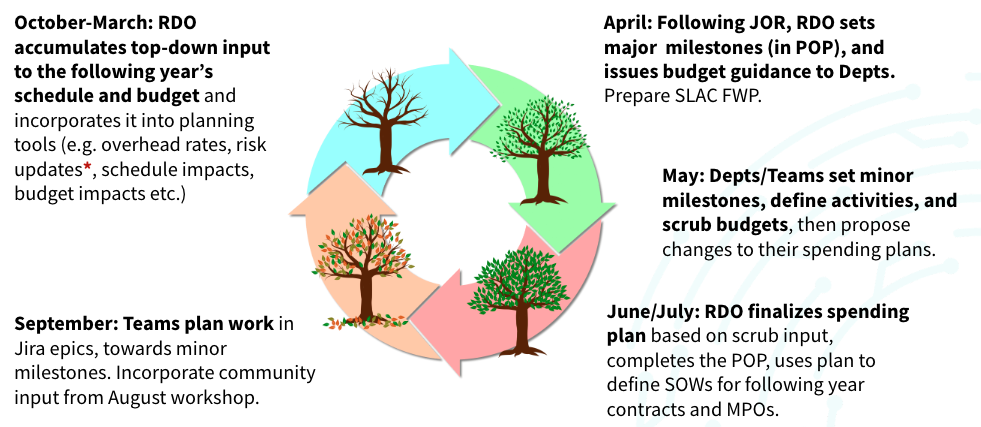
\includegraphics[width=0.95\linewidth]{figures/annual-budget-cycle.png}
\caption{Annual budget planning \gls{cycle}.}
\label{fig:annual-cycle}
\end{figure}


\subsection{Risk-aware budgeting and Requests Beyond Target}

The ground-up spending plan developed during the annual \gls{cycle} is to cover operations work defined by the milestone activities, as well as any regular work captured in bucket epics.
This work includes mitigation of risks held by the teams, as described in the response plans in the risk register.
Any risks that are realized during the year will require action that is not budgeted for.
Additional spending to address realized risks is enabled by Rubin's request beyond target (\gls{RBT}) process, whereby reserve funds are released for use by the departments in response to a specific mid-year request made in a custom Jira ticket.

Standard terminology for financial reserves is that ``management reserve'' describes funds held back to pay for the unknown unknowns, while ``contingency reserve'' is used for known unknowns (i.e.\ the risks in the risk register).
Rubin \gls{Operations}' two funding agencies offer differing guidelines on how reserve should be managed.
DOE allows reserves to be built up and carried forward at \gls{SLAC}, and used as both contingency and management reserve.
DOE \gls{HEP} holds additional reserves centrally, which can also be used as both contingency and management reserve.
NSF \gls{AST} allows line item budget over-estimation by up to 10\%, to allow for increases in cost.
These generate carry-forward (along with any other under-spending that may occur), which we use as contingency reserve.
NSF holds management reserve centrally, to handle unexpected events.

The cost impact analysis of the \gls{Rubin Operations} risk register informs the level of contingency reserve needed.
Residual (post-mitigation) cost exposure for each risk is computed by taking the  product of the residual probability of the risk being realized (in any given year) and the likely annual cost of addressing that risk.
The total cost exposure is then the sum, over all risks in the register, of these products.
While Rubin holds a number of potentially very costly risks, these are generally very unlikely to occur.

Currently, the total cost exposure, and hence the needed level of contingency reserve, is expected to be approximately 15\% of the total annual operating budget at each operations partner.
Included in the risk register is the risk of federal funding allocations being reduced, with a likely cost (if realized in any given year) of some \$1.5M per operations partner.
(At \gls{SLAC}, for example, this would cover about 7\% of the operating expense -- enough to pay the labor bills during a 1 month funding allocation delay.)

Reserve maintenance is accounted for in our federal budget requests, either as an explicit difference between cost and budget on the \gls{DOE} side, or as line by line allowances for increases in cost on the \gls{NSF} side.
At both operations partners carry forward is maintained from one year's plan to the next, with it being spent down to zero either during the post-operations period (at \gls{SLAC}), or before the end of each 5-year renewal period at \gls{NOIRLab}.
Each year a plan is described in the \gls{NOIRLab} \gls{POP} for how carry forward is allocated.
(The restriction on carrying forward funds between renewal periods means that the level of reserve held at \gls{NOIRLab} varies significantly over the course of the 5 years.
Risks that are realized early in the 5-year period are more likely to need supplemental funding from \gls{NSF}'s centrally-held reserves than those that are realized later on, when the carry-forward has been built up.
It may be possible to purposefully hold back scope so as to build up the carry-forward quickly at the start of a renewal period.)

An \gls{RBT} is typically made by a department in order to address risks and/or opportunities as they are realized.
If approved, the \gls{RBT} leads to a draw on the reserve held at one of the operations partners.
(At \gls{NOIRLab}, carry-forward use must be declared a year in advance in the \gls{POP}: this is why the sandboxing process includes a request that the operations teams pitch RBTs for the coming year at that stage.)
The \gls{RBT} itself is a Jira ticket submitted by a department's management team on behalf of the team that is addressing the risk.
Review is by the Directorate team, as budget holders.
The spending associated with an approved \gls{RBT} is not captured in a change to the labor or non-labor plan (which together define the baseline spending plan), but instead is tracked as a variance relative to those plans.

% ======================================================================
\section{Personnel}

\subsection{Staffing Changes}
\label{sec:staffing}

In addition to onboarding procedures at your local institution, please
be aware of

\begin{itemize}
\item The \gls{LSST} \href{https://project.lsst.org/onboarding}{New Employee
  Onboarding} material, and
\end{itemize}

and direct new recruits to them when they join your team\footnote{As per \S\ref{sec:newcomers}, remember that newcomers should be allocated \glspl{SP} for working through this material.}.

The responsible hirere must also complete an \href{https://project.lsst.org/onboarding/form}{onboarding form} for the new recruit.
When members of staff team leave the project, the \gls{T/CAM} should fill in an \href{https://project.lsst.org/onboarding/offboarding_form}{offboarding form}.


% ======================================================================
\section{Open issues}

\begin{itemize}
\item Kanban for \gls{LOE} operations work
\item Need section on more procedural driven work on mountain and \gls{DF}.
\end{itemize}


% ======================================================================
